
\section{Benchmark Evaluation}
\label{sec:micro}

In this section we evaluate the heterogeneous implementation of our 
interface using several micro-benchmarks that test whether our implementation
approaches the underlying performance of the
hardware, and show that the optimizations described in Section~\ref{sec:impl}
are important.  All experiments were run on the Keeneland
supercomputer\cite{Keeneland}.  Each Keeneland node is composed of
two Xeon 5660 CPUs, three Tesla M2090 GPUs, and 24 GB of DRAM.  Nodes
are connected by an Infiniband QDR interconnect.

\subsection{Event Latency and Trigger Rates}
\label{subsec:eventmicro}
We implemented two micro-benchmarks for evaluating the performance of
events.  The first micro-benchmark tests the latency of event triggering,
both within a node and between nodes.  Processors are organized
into a ring and each processor in turn creates a user event that is dependent
on the previous processor's event.  The first event in this long chain of
dependent events is then triggered, and the time until the triggering of the
last event in the chain is measured.  The total time is divided by the number
of events in the chain to yield the mean trigger time.  In the single-node case, all events are local to
that node, so no active messages are required.  For all other cases, the
ring uses only a single processor per node so that every trigger requires
the transmission (and reception) of an event trigger active message.

%% is constructed.  The experiment measures the time from the triggering
%% of the first event to the triggering of the last event.  In the one node
%% configuration there is only one processor and all events are local to the
%% node.  In all other cases, there is only one processor per node which
%% guarantees that all event triggers result in an active message.  
%% Table~\ref{tab:eventlat} shows the results for both configurations.

\begin{figure}
\begin{center}
{ \small
\begin{tabular}{m{2cm}|c|c|c|c|c}
Nodes & 1 & 2 & 4 & 8 & 16 \\ \hline
Mean Trigger Time ($\mu$s) & 0.329 & 3.259 & 3.799 & 3.862 & 4.013 \\
\end{tabular}
}
\end{center}
\vspace{-6mm}
\caption{Event Latency Results.\label{tab:eventlat}}
\vspace{-4mm}
\end{figure}

\hyphenation{GASNet}

The calculated mean trigger times are shown in Table~\ref{tab:eventlat}.
The cost of manipulating the data structures themselves and running dependent
operations is shown by the single-node case, which experienced an average
latency of only 329 nanoseconds.  The addition of nearly 3 microseconds when
going from one node to two can be attributed to the latency of a GASNet
active message; others have measured similar latencies\cite{GASNET06}.
The gradual increase in latency with increasing node count is likely 
related to the underlying point-to-point nature of Infiniband communication,
which requires GASNet to poll a separate connection for every other node in
the system.
%% In the single node case the latency of triggering an event is only 
%% 329 nano-seconds.  For the multi-node cases, the triggering time is
%% between 3-4 micro-seconds which is the same as the cost of GASNet
%% active messages on Infiniband\cite{GASNET07}.  The gradual increase in latency with
%% node count is because each node must poll all the Infiniband connections for other nodes.
%% This cost of performing event triggers is in entirely in the hardware and the underlying software stack.

Our second micro-benchmark for events measures the maximum rate at which events can
be triggered by our implementation.  Instead of a single chain, many parallel chains
are created.  Additionally, each step of the chain consists of a parameterized number
of events, each one dependent on every event from the previous step of the chain.
This parameter is called the {\em fan-in/out factor}.  The events within each step of
a chain are distributed across the nodes.  Recall from Section~\ref{subsec:eventimpl}
that the aggregation of event subscriptions
will limit the number of event trigger active messages to one per node (per event trigger)
even when the fan-in/out factor exceeds the node count.

%% triggers.  This benchmark creates {\em levels} of events where every event at a level
%% corresponds to a merge of all of the events at the previous level.  The benchmark is therefore
%% characterized by the number events at each level called the fan-in/out factor.  
%% The events at each level are evenly distributed between the processors in the machine.
%% In the case of an $n$-node experiment, only $n-1$ active messages will be required 
%% per event trigger because the event subscription mechanism described in 
%% Section~\ref{subsec:eventimpl}.  Figure~\ref{fig:eventthroo} shows the event triggering
%% throughput versus total nodes for a range of fan-in/out factors.

\begin{figure}
\begin{center}
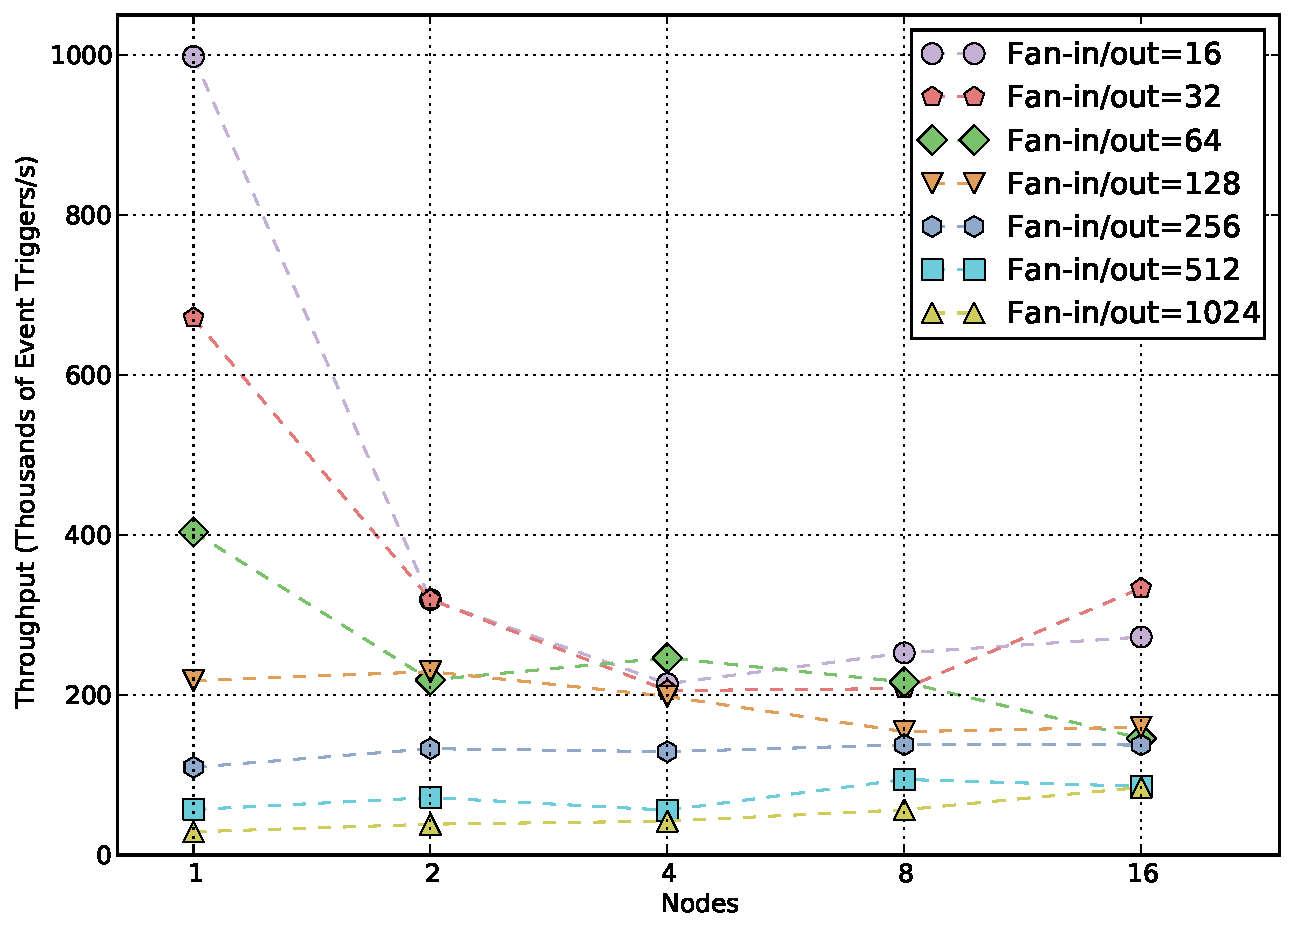
\includegraphics[scale=0.33]{figs/event_throughput.pdf}
\end{center}
\vspace{-6mm}
\caption{Event Trigger Rate Micro-Benchmark.\label{fig:eventthroo}}
\vspace{-4mm}
\end{figure}

Figure~\ref{fig:eventthroo} shows the event trigger rates achieved by our implementation
for a variety of node counts and fan-in/out factors.
For small fan-in/out factors, the total rate falls off initially going to two nodes as active
messages become necessary, but starts increasing slightly again at larger node counts.  Higher
fan-in/out factors require more messages and have lower throughput that also increases with
node count.  Although the number of events waiting on each node decreases with an increasing
node count, the minimal scaling indicates that the main bottleneck is in the processing of the
active message that each node must receive rather than the local redistribution of the triggering
notification.
%Note we can further improve performance by increasing
%the number of threads per node for handling active messages (in these experiments there
%is one per node), but in real applications these threads would consume hardware cores and
%take away computational resources from the primary application.  This is only a viable
%option for memory or communication bound programs.  

The compute-bound nature of the benchmark demonstrates that active messages do not tax 
the interconnection network and leave bandwidth available for application data movement.  
The event trigger rates achieved in this micro-benchmark are between one and two orders
of magnitude larger than the actual trigger rates required by the real applications
described in Section~\ref{sec:apps}.

\subsection{Deferred Lock Grant Rates}
\label{subsec:lockmicro}

Our lock micro-benchmark is designed to measure the rate at which deferred locks can be granted
in a distributed environment.
A parameterized number of locks are created per node and their handles are made available to
every node.  Each node then creates a parameterized number of {\em chains} of lock/unlock
request pairs, where each request pair is to a random lock, and is made dependent on the 
previous lock/unlock pair's completion by the event returned from the lock request.  
The chains are made long enough that start-up
and cleanup times are negligible.  The total number of chains across all nodes gives the total
number of lock requests that can exist in the system at any given time.  All chains are
started at the same time (via a dependence on a single user event), and the total time to
process all the chains is divided into the total number of lock requests to yield an average
lock grant rate.

%% maximum throughput of lock
%% grants.  The benchmark is characterized by the number of nodes, the number
%% of locks initially created by each node, and the number of {\em chains} of
%% lock requests per node.  A chain is 1024 lock acquire and release operations that
%% are serialized by event dependences.  Each node creates the specified number of locks and
%% informs all other nodes of its lock handles.  All nodes create the specified number
%% of chains by randomly selecting from the set of all locks in the system.  All chains
%% are predicated on a user event.  The experiment measures the time from the triggering of
%% the user event to the completion of all chains.

Figure~\ref{fig:fixedlock} shows the lock grant rate for a variety of node counts and locks
per node.  The number of chains per node is varied so that the total number of chains in the system
is 1024 in all cases.  For the single-node cases, the insensitivity to the number of locks indicates
that the bottleneck is in the computational ability of the node to process the requests. 
For larger numbers of nodes, especially for the larger numbers of locks per node (where contention
for any given lock is low), the speedup with increasing node count suggests the limiting factor is
the rate at which lock-related active messages can be sent (nearly every request will require a
transfer of ownership).  Especially in the middle of the node count range, the performance actually
increases with
decreasing lock counts.  Although contention increases, the favoring of local lock requestors makes
the contention an advantage, reducing the number of lock-related active messages that must be sent
per lock grant.

%%  When going
%% from one node to two nodes, the bottleneck becomes the latency of transferring ownership of locks
%% between the nodes
%%  versus nodes in the system
%% for 256 total chains in the system.  Each line corresponds
%% to a different number of initial locks per node.  At small node counts, 
%% small numbers of locks per node cause high
%% contention and lock unfairness allows for very high throughput as many requests are
%% handled locally before locks are migrated.   When there are more total locks there
%% is lower contention and lower throughput because the ratio of lock grants to migrated
%% locks decreases.  At larger node counts, there are enough locks
%% in the system to remove contention and throughput improves.

\begin{figure}
\begin{center}
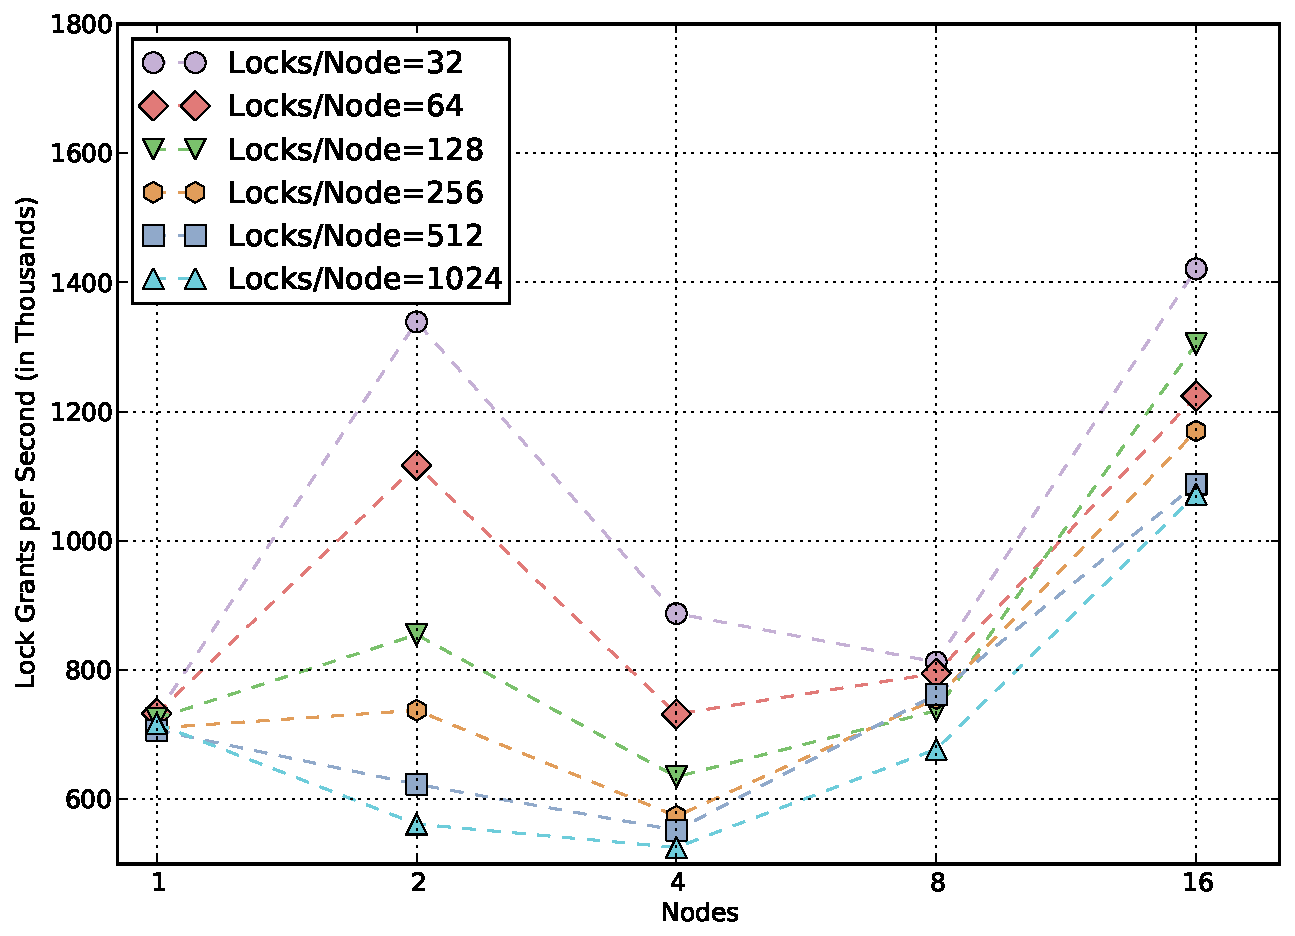
\includegraphics[scale=0.33]{figs/fixed_lock_chains.pdf}
\end{center}
\vspace{-6mm}
\caption{Lock Benchmark for Fixed Total Chains.\label{fig:fixedlock}}
\vspace{-4mm}
\end{figure}

To more clearly demonstrate the benefit of lock unfairness, even at large node counts, we show an alternative
cut of the experiment space in Figure~\ref{fig:fixednode}.
In this case the node count is fixed at 8 and lock grant rates are shown for a variety of total lock counts
and number of chains per node.
With only 32 chains per node (a total of 256 chains)
there is little contention and the grant rate is high.  As the number of chains per node increases there is
more contention for locks and the rate drops as a result.  For smaller lock counts, further increases in
the number of chains result in improved rates.  Note that the point on each line where the increase occurs
is when the chains per node is greater than total locks, which corresponds to the point where the expected 
number of requests per lock 
per node becomes more than one.  As soon as there are multiple expected requestors for the same lock on
a node, the unfairness property of our lock implementation is able to reduce the number of lock ownership 
transfers, yielding better performance.

\begin{figure}
\begin{center}
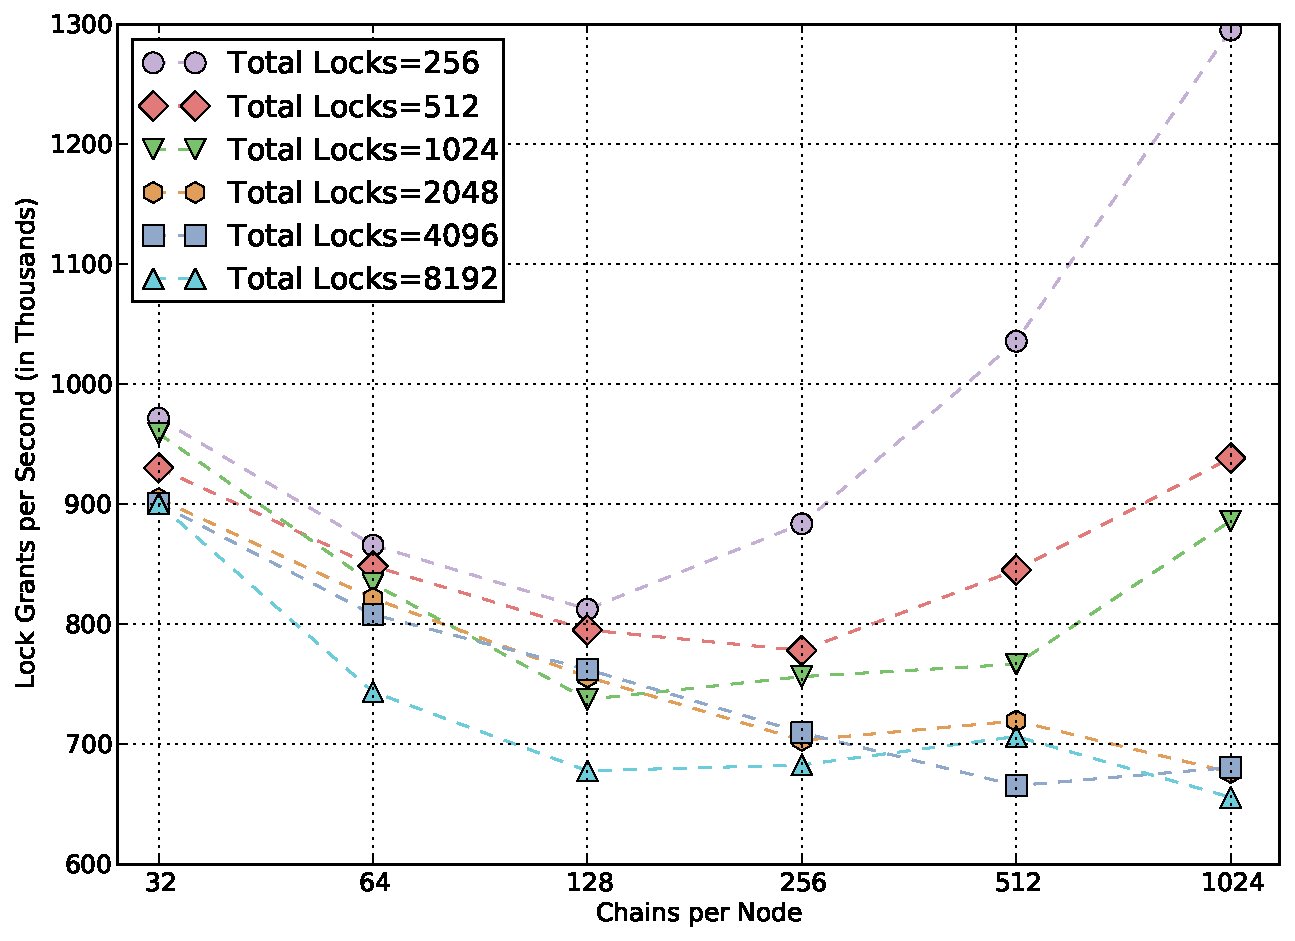
\includegraphics[scale=0.33]{figs/fixed_node_lock.pdf}
\end{center}
\vspace{-6mm}
\caption{Lock Benchmark for Fixed Node Count.\label{fig:fixednode}}
\vspace{-4mm}
\end{figure}


\subsection{Reduction Throughput}
\label{subsec:reducmicro}
To show the benefits of reduction instances we designed
a histogram micro-benchmark that requires all nodes to perform an addition reduction to a
physical region located in the globally visible GASNet memory (described in 
Section~\ref{sec:impl}).  Using the reduction interface described in Section~\ref{subsec:phyreg}
reductions are performed in five ways:

\begin{itemize} \itemsep1pt \parskip0pt \parsep0pt
\item Single Reads/Writes - Each node takes a lock on the global physical region and then for each reduction
reads a value from the physical region, performs the addition, and then writes the result back.  The lock is then released.
\item Single Reductions - Each reduction is individually sent as an active message to the node whose
system memory holds the target of the reduction.
\item Localized Instance - Each node takes a lock on the the global physical region, copies it to a new physical
region in its own system memory, performs all reductions to the localized region, copies the region back, and releases the lock.
\item Fold Instance - Each node creates a local fold reduction instance.
All reductions are folded into the instance, which is then copied back to the global region.
\item List Instance - Each node creates a local list reduction instance.
All reductions are appended to the list reduction instance, which is then copied back to the global region.
\end{itemize}

We ran two experiments, one corresponding with dense reductions and the other corresponding with sparse
reductions.  In each case a large random source of data is divided into chunks, which are given to
separate reduction tasks.  There are 8 reduction tasks created for each node, one per processor.  The dense
case uses a histogram with 256K buckets and each reduction task performs 4M reductions.  The results for the
dense experiment are shown in Figure~\ref{fig:reducdense}.  The sparse case uses a histogram with 4M buckets,
but only 64K reductions are performed by each task.  Results for the sparse case
be seen in Figure~\ref{fig:reducsparse}.

The dense experiment demonstrates that reduction fold regions perform 
best and scale well with the number of nodes, achieving over a billion reductions
per second in the 16 node case.  List regions also scale well, but perform about an
order of magnitude worse than folding regions in the dense case.  The use of a separate active message for
each reduction operation is another two orders of magnitude worse, demonstrating that data must be
transferred in larger blocks to be efficient on modern interconnect hardware.  The localized instance approach
works well for a single node, but its inherently serial nature doesn't benefit from increasing node counts.  Finally, the only time the latency of performing individual RMA reads and writes isn't disastrous is
on a single node (where the reads and writes are all local).

The sparse case is very similar, except the scalability of the reduction fold case suffers from the
overhead of transferring a value for every bucket when most buckets are unmodified by a given task.
The reduction list case continues to scale well, surpassing the reduction fold performance at large
node counts.  This shows that
list regions are better suited for scaling sparse reduction operations.

\begin{figure}
\begin{center}
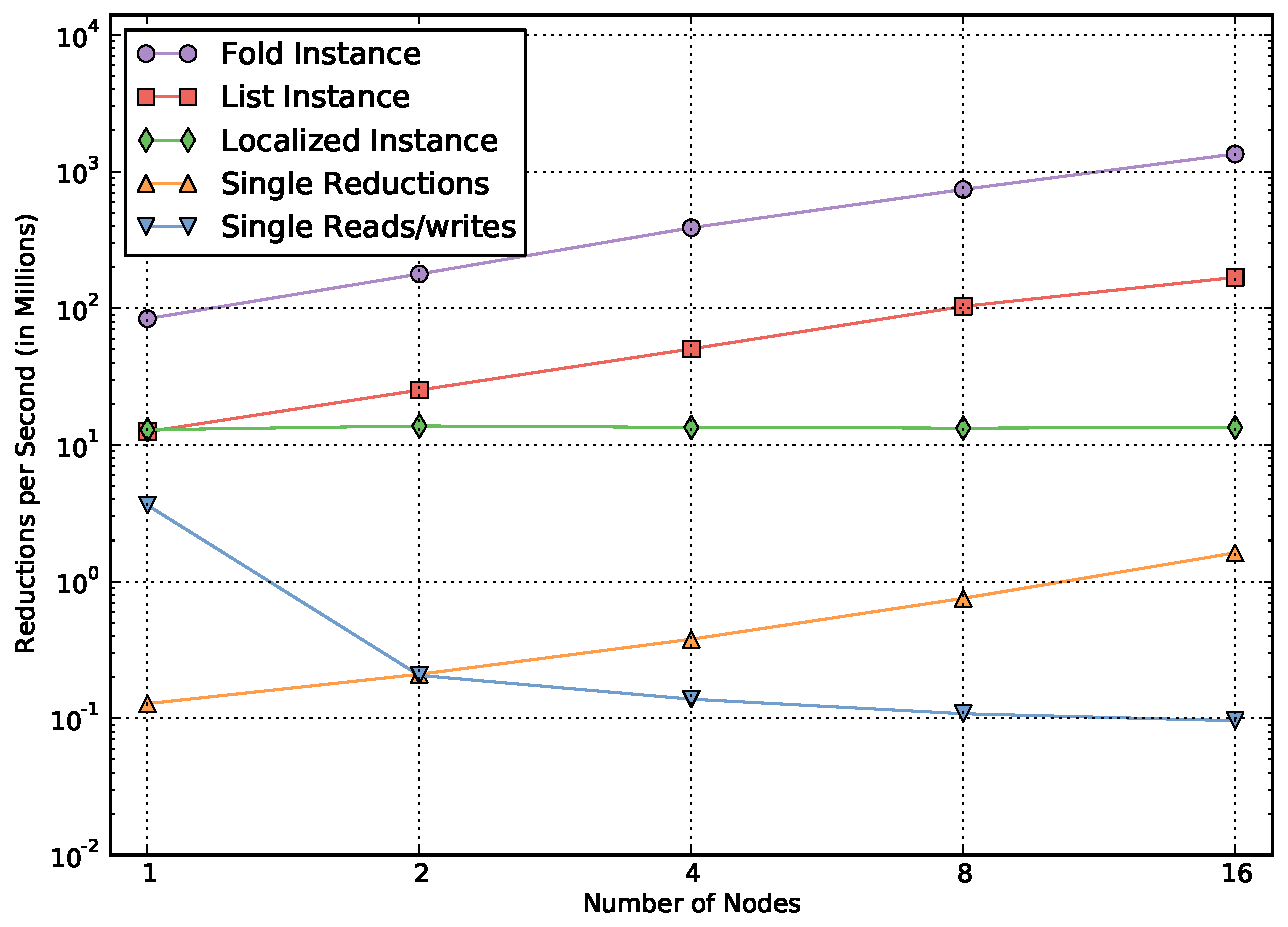
\includegraphics[scale=0.33]{figs/reduce_dense.pdf}
\end{center}
\vspace{-6mm}
\caption{Dense Reduction Benchmark.\label{fig:reducdense}}
\vspace{-4mm}
\end{figure}

\begin{figure}
\begin{center}
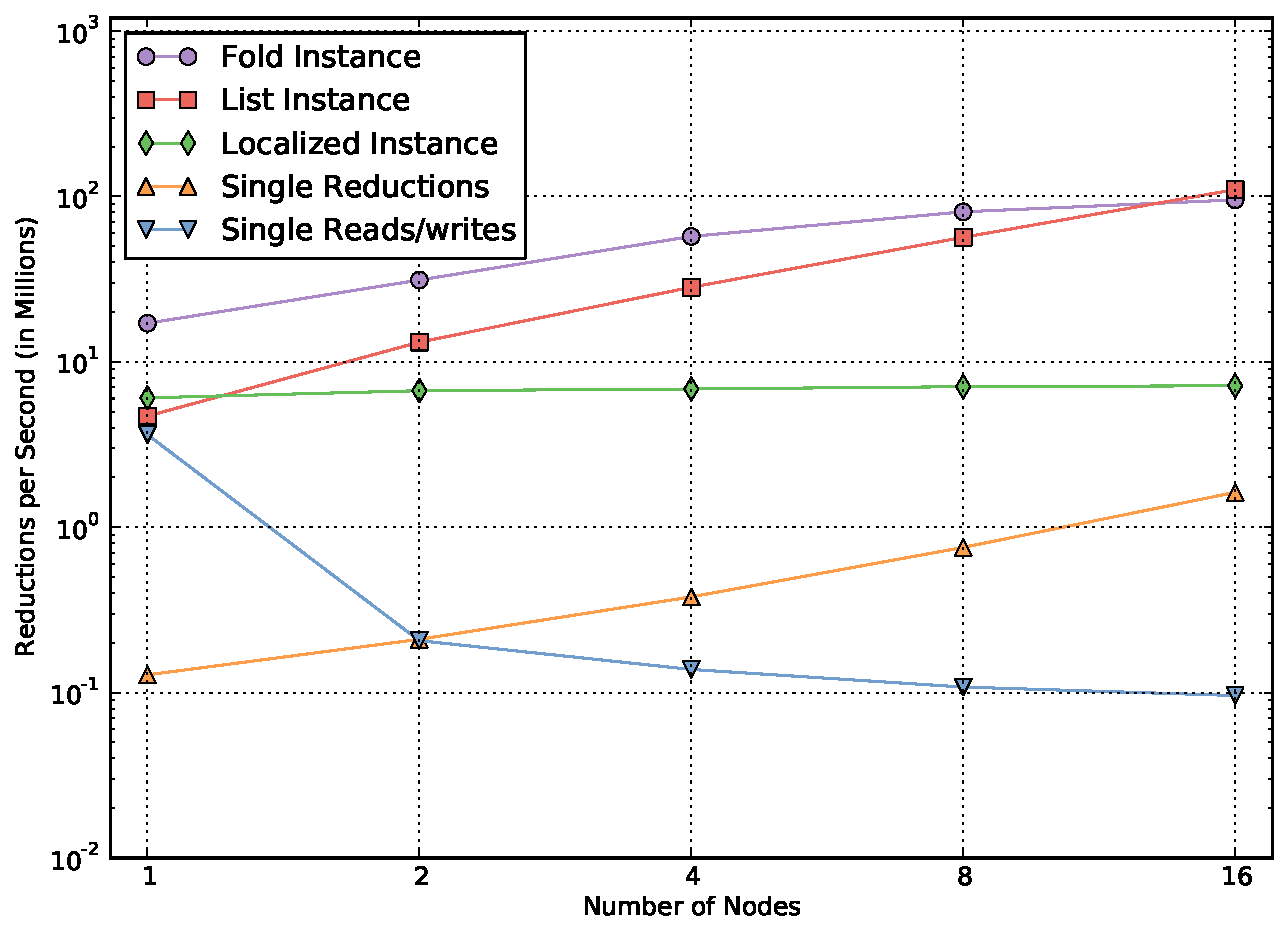
\includegraphics[scale=0.33]{figs/reduce_sparse.pdf}
\end{center}
\vspace{-6mm}
\caption{Sparse Reduction Benchmark.\label{fig:reducsparse}}
\vspace{-4mm}
\end{figure}

